%-----------------------------------------------------------------------------
%
%               Template for sigplanconf LaTeX Class
%
% Name:         sigplanconf-template.tex
%
% Purpose:      A template for sigplanconf.cls, which is a LaTeX 2e class
%               file for SIGPLAN conference proceedings.
%
% Guide:        Refer to "Author's Guide to the ACM SIGPLAN Class,"
%               sigplanconf-guide.pdf
%
% Author:       Paul C. Anagnostopoulos
%               Windfall Software
%               978 371-2316
%               paul@windfall.com
%
% Created:      15 February 2005
%
%-----------------------------------------------------------------------------


\documentclass{sigplanconf}

% The following \documentclass options may be useful:

% preprint      Remove this option only once the paper is in final form.
% 10pt          To set in 10-point type instead of 9-point.
% 11pt          To set in 11-point type instead of 9-point.
% authoryear    To obtain author/year citation style instead of numeric.

\usepackage{usenix,epsfig,endnotes}
\usepackage{xcolor}
\usepackage{xspace}
\usepackage{hyperref}
\usepackage{listings}
\usepackage{subfig}

\begin{document}

\special{papersize=8.5in,11in}
\setlength{\pdfpageheight}{\paperheight}
\setlength{\pdfpagewidth}{\paperwidth}

\conferenceinfo{CONF 'yy}{Month d--d, 20yy, City, ST, Country} 
\copyrightyear{20yy} 
\copyrightdata{978-1-nnnn-nnnn-n/yy/mm} 
\doi{nnnnnnn.nnnnnnn}

% Uncomment one of the following two, if you are not going for the 
% traditional copyright transfer agreement.

%\exclusivelicense                % ACM gets exclusive license to publish, 
                                  % you retain copyright

%\permissiontopublish             % ACM gets nonexclusive license to publish
                                  % (paid open-access papers, 
                                  % short abstracts)

%\titlebanner{banner above paper title}        % These are ignored unless
%\preprintfooter{short description of paper}   % 'preprint' option specified.

\title{\Large \bf High-Performance Determinism with Total Store Order Consistency}
%\subtitle{Subtitle Text, if any}

%\authorinfo{Name1}
%           {Affiliation1}
%           {Email1}
%\authorinfo{Name2\and Name3}
%           {Affiliation2/3}
%           {Email2/3}

\maketitle


\newcommand{\checkout}{{\tt checkout()}}
\newcommand{\settled}{{\tt commit()}}
\newcommand{\settledm}{{\tt commit\_mutex()}}
\newcommand{\update}{{\tt update()}}
\newcommand{\updatem}{{\tt update\_mutex()}}
\newcommand{\commit}{{\tt commit()}}
\newcommand{\commitm}{{\tt commit\_mutex()}}
\newcommand{\mksnap}{{\tt commit()}}
\newcommand{\getsnap}{{\tt update()}}
\newcommand{\fork}{{\tt fork}}
\newcommand{\pte}{{\tt pte}}
\newcommand{\determEnd}{{\tt determ\_end}}
\newcommand{\pthread}{{\tt pthread}}


\newcommand{\create}{{\tt pthread\_create}}
\newcommand{\dthreads}{Dthreads}



\newcommand{\conversion}{{\sc \small Conversion}}
\newcommand{\lib}{{\sc \small Consequence}\xspace}
\newcommand{\libnodet}{{\sc \small Consequence-NoDet}\xspace}
\newcommand{\Lib}{{\sc \large Consequence}\xspace}

\newcommand{\TODO}[1]{\textbf{\textcolor{red}{[ TODO: #1]}}}


\begin{abstract}

We present \lib{}, a high performance deterministic multi-threading library. 
\lib{} achieves deterministic execution through store buffering and strict ordering of synchronization operations.
To ensure high performance under a wide variety of conditions, the ordering of synch operations is based on a deterministic clock \cite{olszewski_kendo:_2009}, 
and store buffering is implemented using version-controlled memory \cite{merrifield_conversion:_2013}.

While recent work on deterministic concurrency \cite{devietti_rcdc:_2011,kai_lu_efficient_2014} has proposed relaxing the consistency model beyond total store ordering (TSO), the runtime performance of such methods is so far unclear, and memory requirements of 5--50$\times$ pthreads have been reported\cite{kai_lu_efficient_2014}.
Meanwhile, we demonstrate that benchmark runtimes within $2.5\times$ of pthreads is achievable with TSO, given an abstract, optimal ordering. Finally, we provide a concrete ordering that achieves a maximum slowdown of 3.1$\times$ vs. non-deterministic pthreads, across 12 benchmarks in the Phoenix and PARSEC benchmark suites.

\end{abstract}


\section{Introduction}

With multi-core processors comes the need for parallel programs. 
%Along with the profusion of multi-core processors over the last decade has come the need for parallel software that can take advantage of these new architectures. 
%Unfortunately, writing parallel software that is both correct and performs well is hard still an open challenge. 
%Writing sequential software that is correct and performs well is hard enough.
Unfortunately, writing parallel programs is hard. 
On top of the difficulties of writing correct sequential programs, parallelism brings nondeterminism which undermines our ability to debug, test and understand our programs.

%In recent years many researchers have proposed ways to execute general parallel programs deterministically without sacrificing much parallelism or performance. 
Research into deterministic concurrency seeks to alleviate these problems. %has seen much progress in recent years.
While some initial proposals focused on the design of deterministic multi-core architectures \cite{devietti_dmp:_2009,devietti_rcdc:_2011,derek_r._hower_calvin:_2011}, subsequent work has demonstrated practical pure-software implementations of determinism  \cite{liu_dthreads:_2011,merrifield_conversion:_2013,kai_lu_efficient_2014}.

One of the central techniques for improving performance in both hardware and software deterministic systems has been relaxing the memory consistency model. While initial proposals adopted strong consistency models like sequential consistency \cite{devietti_dmp:_2009} and total store order (TSO) \cite{bergan_coredet:_2010}, subsequent work relies on extremely relaxed consistency models like DRF0 \cite{devietti_rcdc:_2011} and lazy release consistency (LRC) \cite{kai_lu_efficient_2014} to reduce inter-thread communication and thus improve performance.
%for good performance.% Weakening the consistency model admits better scalability by allowing memory fences to coordinate with a subset of threads instead of with all threads \cite{devietti_rcdc:_2011,kai_lu_efficient_2014}. 
%Relaxed consistency allows fences to perform localized work instead of the global coordination required by strong consistency models. 
However, all deterministic execution systems, relaxed consistency or not, require global ordering of inter-thread communication, a likely bottleneck in any deterministic concurrency system. 
%This can be abstracted as a deterministic logical clock (DLC), based on synchronization operations \cite{liu_dthreads:_2011} or instruction counting \cite{olszewski_kendo:_2009, devietti_dmp:_2009}, where the thread with the lowest clock has priority.
%Our system, \lib, also implements a deterministic logical clock which inherently requires global coordination (\S\ref{s:dlc}). 
%Our insight is that optimizing the implementation of memory fences is of limited benefit when other global bottlenecks remain. 
We argue that while this bottleneck remains, relaxing the consistency model is of limited benefit. 
Moreover, the adoption of an extremely relaxed consistency model is not free. Supporting LRC, as \cite{kai_lu_efficient_2014} does, suffers from high space overheads that hinder scalability. The programmability challenges inherent in relaxed consistency are also well-known, and can result in unintuitive behavior \cite{adve_data_2010,batty_mathematizing_2011}. Finally, some current hardware memory consistency models like x86 are not as relaxed as LRC. Moving to a weaker consistency model breaks compatibility with existing binaries. In contrast, a system that offers consistency guarantees compatible with modern architectures can support legacy binaries simply by replacing the pthreads library.

% The core issue is that a program that "works" on TSO can break on LRC. Consider flag-based synchronization with locking where the sender uses lock A and the receiver uses (by mistake) lock B. Due to the global nature of commits, this will still work on TSO but will deadlock on LRC. There's a data race in the program so any semantics are permissible, but there is a practical consideration as well that we shouldn't break code that already works.

\lib demonstrates that a deterministic implementation of TSO, a relatively strong consistency model that is compatible with all modern hardware platforms, can perform well across a range of workloads. The primary contributions of this paper are:
\begin{itemize}
%\item We identify that deterministic synchronization is a global bottleneck affecting all deterministic execution schemes, regardless of consistency model.
\item We describe several TSO-compatible optimizations that target the same scenarios that relaxed consistency optimizes, reducing the scope for further improvements from relaxed consistency.
\item We demonstrate deterministic adaptation to program behavior as a means of further improving performance.
%\item We describe a novel implementation of deterministic locking that supports blocking instead of polling.
\item We describe novel implementations of deterministic synchronization operations that are flexible and increase the parallelism of prior techniques.
\item Finally, we demonstrate a deterministic implementation of TSO that achieves a 2.8x and 2.2x improvement over DThreads \cite{liu_dthreads:_2011} and DWC \cite{merrifield_conversion:_2013} (respectively) on the five most challenging benchmark programs.

\newpage

\end{itemize}
While determinism can simplify parallel programming, using complicated memory consistency models to make determinism fast under-cuts these programmability gains. \lib erases this tension by combining determinism and strong memory consistency.

% PLACE HOLDER UNTIL WE HAVE A BETTER PRETTY CONCLUDING PARAGRAPH... 
% Below, we describe and motivate the \lib{} design (\S\ref{s:perf}) and several key optimizations (\S\ref{s:optimizations}). \S\ref{s:sync} describes our deterministic synchronization operations, followed by evaluation (\S\ref{s:eval}), related work (\S\ref{s:related}) and conclusions (\S\ref{s:concl}). 

%%% Local Variables: 
%%% mode: latex
%%% TeX-master: "paper.tex"
%%% End:

\section{\Lib{}: Background, Design and its Motivation}
\label{s:perf}

Current deterministic execution systems \cite{liu_dthreads:_2011,merrifield_conversion:_2013,kai_lu_efficient_2014} allow an arbitrary multi-threaded program written in a conventional parallel programming language (like C or Java) to execute in a deterministic manner (the \emph{singleton} definition of determinism \cite{Lu:2011:DISC}). The program's output and succession of internal states become solely a function of the program's explicit inputs 
and are unaffected by the non-deterministic interleaving of shared memory operations or scheduler policy.

\lib{} is intended as a high-performance, deterministic, drop-in replacement library for pthreads. Any pthreads-compatible program may be linked with \lib{} to create a deterministic, yet efficient version of the same. Determinism is assured for all programs, even those with data races. However, the use of atomic instructions or ad-hoc synchronization methods such as spinning on flag variables may (deterministically) result in incorrect behavior (\S\ref{s:adhoc}). Further, in order to ensure correctness memory conflicts are merged at a byte granularity. In the presence of data races, this can result in outcomes not possible in non-deterministic execution \cite{kai_lu_efficient_2014}. In these aspects \lib{} offers the same determinism and progress guarantees as other recent deterministic execution systems \cite{liu_dthreads:_2011,kai_lu_efficient_2014}. In contrast with some prior work \cite{olszewski_kendo:_2009}, \lib{} does not assume that programs are race-free.

We now briefly summarize the design of \lib{}.
To achieve determinism, \lib{} uses a deterministic, instruction-count based logical clock (\S\ref{s:dlc}), and memory isolation using page table manipulation and deterministic, byte-level merging at synchronization points (\S\ref{s:commit}). All pthreads synchronization operations are replaced with deterministic equivalents, which ensure a strict ordering of these operations (\S\ref{s:detsync}) based on the logical clock. \lib{} also supports ad-hoc synchronization through periodically (and deterministically) synchronizing memory in the absence of explicit synchronization operations (\S\ref{s:adhoc}). 

Below, we provide background on deterministic concurrency, and describe and motivate each of the design choices made in \lib{}.

All deterministic execution schemes must provide two key components: 1) a \emph{deterministic logical clock} to enforce a deterministic order of synchronization operations and 2) a \emph{deterministic memory consistency model} that ensures loads return deterministic values even in the presence of unsynchronized accesses. Together, these two components are sufficient to guarantee the determinism of arbitrary programs. Below, we present and motivate the primary decisions that guided the design of \lib{}, while reviewing the alternative designs used in prior work.

\subsection{Deterministic Logical Clocks}
\label{s:dlc}

A deterministic logical clock is a mechanism that provides a deterministic total ordering for synchronization operations. A total order is necessary because synchronization operations must be globally coordinated in the general case when the system has no knowledge of what synchronization threads may attempt to perform next. The deterministic logical clock must ensure that, e.g., if two threads try to acquire the same lock, the same thread always wins. 

\begin{figure}
\centering
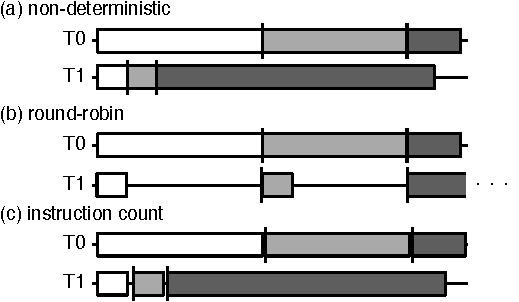
\includegraphics[width=3.0in]{figures/sync-frequency.pdf}
\caption{Effect of mismatched rate of synchronization operation. Vertical bars--sync. ops, boxes--work performed. (a) Mismatch causes no waiting with non-deterministic execution, but (b) can incur extensive waiting with round-robin deterministic logical clocks. (c) An instruction-count based logical clock \cite{olszewski_kendo:_2009} incurs waits close to those of a non-deterministic system. }
\label{f:sync-freq}
\end{figure}

The simplest logical clock is a round-robin policy and has been proven to work well in many prior schemes \cite{devietti_dmp:_2009,bergan_coredet:_2010,derek_r._hower_calvin:_2011,liu_dthreads:_2011,merrifield_conversion:_2013}. The round-robin policy works well when threads perform synchronization operations at the same rate. However, a thread that performs synchronization operations frequently can end up spending most of its time waiting for a thread that synchronizes rarely (\autoref{f:sync-freq}b).

A more efficient policy was proposed in Kendo \cite{olszewski_kendo:_2009} where the number of user instructions retired determines the deterministic ordering. The number of retired instructions may be determined using either performance counters \cite{olszewski_kendo:_2009,devietti_rcdc:_2011} or compiler instrumentation \cite{kai_lu_efficient_2014}. Under this design, a deterministic total ordering is obtained by allowing only the thread with the global minimum instruction count (GMIC) to perform a synchronization operation.

If all instructions required the same amount of time to execute, the Kendo approach would produce a very good ordering in the sense that threads would never have to wait long to perform a synchronization operation (\autoref{f:sync-freq}c). However, instruction latencies can vary greatly depending on the particular instruction being executed or non-deterministic processor state (e.g cache). Compounding this issue, the library implementations of deterministic synchronization operations can contain non-deterministic code such as system calls or acquisition of spin locks for internal purposes. To avoid non-determinism, an obvious solution is to disable the instruction counting whenever such code may be executed. Both instruction latency variance and clock disabling can lead to {\it clock skew}, where the logical clock becomes increasingly disconnected from real time.

In \lib{}, we use the retired instruction count for ordering based on hardware performance counters. Threads pass a single \emph{global token} between themselves and the token can only be acquired by the GMIC thread. We mitigate clock skew by allowing clocks to deterministically ``fast-forward'' as described in \S\ref{s:fast-forward}. While we have observed a small degree of nondeterminism in our performance counter measurements (consistent with other work \cite{4636099}) our logical clock is sound in the presence of deterministic performance counters and could also be constructed from lightweight compiler-based instruction counting \cite{kai_lu_efficient_2014}.

\subsection{Deterministic Memory Consistency}

A deterministic memory consistency model ensures that loads from shared memory always return the same value across program runs even in the presence of unsynchronized accesses, i.e., data races. While most loads are well-synchronized, and thus rendered deterministic by deterministic synchronization operations (\S\ref{s:dlc}), unsynchronized loads require additional effort. While \cite{olszewski_kendo:_2009} provides deterministic memory consistency by assuming data-race-free programs, most deterministic consistency models are built around the idea of temporarily isolating each thread in its own memory space. When threads are isolated, a multi-threaded program is effectively converted into a collection of single-threaded programs, each of which are inherently deterministic. Of course, threads must periodically be allowed to communicate with each other. The strength of the memory consistency model determines when a thread's updates, accumulated in isolation, must be made visible to other threads: stronger models require updates to be shared more frequently and more widely than weaker models. The key design decision for deterministic memory consistency is the semantics of a memory fence, the mechanism that controls how updates propagate to remote threads. We refer to the process of making updates visible as a \emph{commit} operation to distinguish it from the hardware's memory fence instructions. While commit operations are not inherently deterministic, they are rendered so by enforcing a commit ordering with a deterministic logical clock (\S\ref{s:dlc}).

\subsection{Total Store Order is Enough}

\begin{figure}
\centering
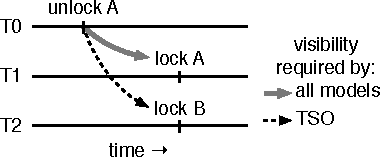
\includegraphics[width=2.7in]{figures/relaxed-consistency.pdf}
\caption{TSO requires that commits are global, while more relaxed models allow local commits that are visible to a subset of threads.}
\label{f:relaxed}
\end{figure}

Relaxing the consistency model improves the performance of determinism by making commits cheaper. Consistency models like sequential consistency and total store order require that stores become visible in a total order that all threads agree on: commits must thus be a global operation visible to all threads (\autoref{f:relaxed}). Relaxed consistency models like DRF0 \cite{devietti_rcdc:_2011} and LRC \cite{kai_lu_efficient_2014} allow commits to be ``point-to-point'' with respect to a given synchronization object, i.e., the commit performed when releasing a lock need be visible only to the thread that subsequently acquires that lock.

While an LRC-based system may in principle offer better performance than a TSO-based system, the adoption of such an extremely relaxed\footnote{It is not obvious how further relaxations beyond LRC would be possible without breaking programming language semantics.} consistency model entails several additional costs. One concern is a space leak that arises from making commits visible only via a particular synchronization object. In \cite{kai_lu_efficient_2014}, if a thread modifies some data and releases lock A, those modifications must be recorded until some other thread acquires lock A. This causes space usage to scale with the number of lock objects. In the case that no other thread ever acquires lock A, space will be permanently leaked. This space overhead is not just a theoretical concern: in \cite{kai_lu_efficient_2014} large space overheads for one LRC-based system restricted the evaluation of some programs to just four threads.

%n \S\ref{s:rfdet} we report \TODO{If we get rid of that section, just cite the RFDet paper} large space overheads for one LRC-based system, on a benchmark with only a moderate number of synchronization operations.

 In addition to its space overheads, weak consistency models like LRC are difficult for both humans \cite{adve_data_2010} and automated tools \cite{batty_mathematizing_2011,burckhardt_checkfence:_2007} to understand. LRC is more relaxed than the TSO consistency models of x86 and SPARC, and thus legacy binaries on those platforms can break when moved to LRC.

\lib{} adopts the TSO consistency model, offering a familiar programming environment and compatibility with binaries compiled for any modern hardware platform. In our evaluation (\S\ref{s:eval}), we demonstrate that efficient determinism is achievable without sacrificing TSO consistency. 

\subsection{Implementing Commits}
\label{s:commit}

While the memory consistency model does somewhat constrain the possible implementations of the commit operation, many alternative designs are still possible for a given consistency model. For instance, several deterministic execution systems implement the TSO consistency model by dividing program execution into chunks consisting of a fixed number of instructions (typically 10,000-100,000) and placing a commit at the end of each chunk \cite{bergan_coredet:_2010,derek_r._hower_calvin:_2011}. Chunks are terminated early if they contain a synchronization operation. However, memory models like TSO do not require commits at places other than synchronization operations. Thus, an even more efficient TSO-based system was proposed in \cite{liu_dthreads:_2011} where chunks are as large as the regions between synchronization operations, i.e., 
commits occur only at synchronization operations. This approach better amortizes the costs of a commit.

\begin{figure}
\centering 
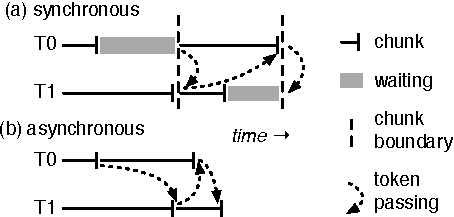
\includegraphics[width=3.0in]{figures/sync-async-chunks.pdf}
\caption{Synchronous versus asynchronous commit.}
\label{f:sync-async}
\end{figure}

Moreover, in all of these systems  \cite{bergan_coredet:_2010,derek_r._hower_calvin:_2011,liu_dthreads:_2011} commits are \emph{synchronous} operations that require coordination among all threads in the program. This synchronous approach (\autoref{f:sync-async}a) can lead to excessive waiting if threads do not naturally want to commit simultaneously.

 An alternative \emph{asynchronous} approach was proposed by \cite{merrifield_conversion:_2013}. Here, instead of a shared workspace, threads share a list of changes, and each thread applies these changes to their own workspace when appropriate. This allows threads to commit independently (\autoref{f:sync-async}b), increasing parallelism. This optimization does not break TSO because updates still appear in a total order that all threads agree on. Indeed, in modern TSO processors memory fences are implemented in a similarly asynchronous fashion.

With \lib we build upon the approach of \cite{merrifield_conversion:_2013}. However, we observe that if the number of instructions between synchronization operations is small the fixed costs of committing cannot be effectively amortized. To counteract this effect \lib{} performs adaptive coarsening of these chunks, dynamically and deterministically selecting a target chunk size to optimize performance. Coarsening does not affect TSO consistency because a fence in TSO does not require that updates be made visible immediately, merely that writes made after the fence appear no sooner than writes made before it. Coalescing multiple commits and making them visible all at once is thus valid under TSO. We provide a more detailed discussion of adaptive coarsening in \S\ref{s:optimizations}.

\subsection{Implementing Thread Isolation}
\label{s:isolation}

Many possible implementations of thread isolation have been explored by prior systems. For example, compiler instrumentation \cite{bergan_coredet:_2010, kai_lu_efficient_2014} can be used to buffer a thread's writes into per-thread store buffers. This approach introduces considerable overhead for each write and requires recompilation of all programs and libraries. Hardware store buffers \cite{devietti_rcdc:_2011,derek_r._hower_calvin:_2011,jooybar_gpudet:_2013} have also been proposed to avoid these overheads. Virtual memory protection hardware on existing systems can also be used to intercept writes on a per-page basis using the {\tt mprotect()} system call \cite{liu_dthreads:_2011} or kernel modifications \cite{merrifield_conversion:_2013}. Using virtual memory techniques requires the use of processes instead of threads.

\begin{figure}
\begin{center}
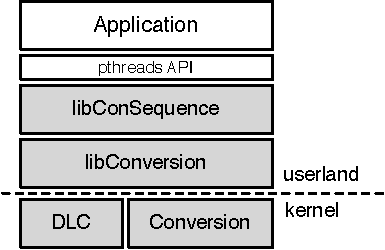
\includegraphics[width=2.2in]{figures/arch}
\caption{\lib{} architecture diagram. Shaded components indicate our system. \lib{} is implemented primarily in the form of a runtime library, but is supported by several key components implemented in the Linux kernel.}
\label{f:arch}
\end{center}
\end{figure}

%The overall architecture of \lib is shown in \autoref{f:arch}.

\lib{}'s implementation of thread isolation relies on \conversion{} \cite{merrifield_conversion:_2013}, a kernel-implemented version control system for main memory segments.
\conversion{} allows a \lib{} thread (actually a process) to operate on a {\it local copy} of a memory segment in complete isolation, until it explicitly retrieves remote changes, or commits its local changes. \lib{} provides deterministic memory consistency for only the globals and heap segments.\footnote{Shared memory segments mapped by the user will not behave deterministically.}

When a thread $T0$ begins a chunk, its globals and heap segments are updated to the latest available version of memory and each page is write-protected.  Writes will trigger a copy-on-write page fault and a reference to the new page will be stored in a thread-local dirty list. On commit, a new version is created that contains the modified pages from the dirty list. If another thread $T1$ has committed since $T0$ began its chunk, it will have to update its page table to reflect those modifications. If there is a page-level conflict (i.e., $T0$ and $T1$ wrote to the same page), a basic byte-granularity merging mechanism enforces a last-writer-wins policy. 

% \subsection{Inter-thread Communication}
% \label{s:asynchronous}

% Once a thread makes it past a synchronization point, it must retrieve any local updates and make its local changes available to other threads. 
% This may be done in one of two ways: in \cite{which}\TODO{Joe: please fill in refs}, threads execute in lock step, alternating between {\it local work} and {\it global coordination}. Under this model, all threads may make modifications directly (but in order) to a shared workspace, which forms the starting point for the next phase of {\it local work} of all threads. \TODO{Joe: is this where you used the terms centralized vs distributed before? seems quite appropriate to me now...} This \emph{synchronous} approach (\autoref{f:sync-async}a) can lead to excessive waiting as threads often execute instructions or synchronization operations at different rates.


\subsection{Deterministic Synchronization}
\label{s:detsync}

The pthreads API defines synchronization operations that are used to ensure the correctness of parallel programs. Any usable determinism system must implement a deterministic version of this API. The main primitives provided are \emph{mutual exclusion}, \emph{condition variables}, and \emph{barriers}. Additional primitives such as thread \emph{create}, \emph{join} and \emph{exit} are also typically handled by deterministic systems. Previous work has varied greatly in its support and implementation of these primitives. In \cite{liu_dthreads:_2011}, the mutual exclusion implementation replaces all locks with a single global lock. This obviously negates any performance benefits gained by fine-grained locking code.

\begin{figure}
\centering
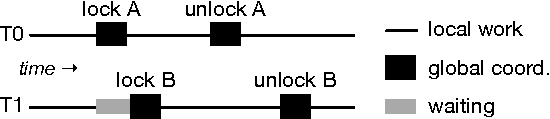
\includegraphics[width=3in]{figures/local-global}
\caption{Global coordination is required only for synchronization operations, not for critical sections.}
\label{f:local-global}
\end{figure}

\lib{} provides efficient implementations of the common pthreads synchronization primitives listed above. Each synchronization primitive is implemented using both the deterministic logical clock (\S\ref{s:dlc}) and commit (\S\ref{s:commit}) mechanisms. While highly relaxed consistency models like LRC can make commits into local operations, clock operations fundamentally require global coordination. Thus, in \lib{}, critical sections protected by different locks constitute local work that can execute concurrently, though the lock acquires and releases themselves require global coordination. In \autoref{f:local-global}, locking A and B invokes global coordination phases which must be serialized. However, between the lock and unlock operations, threads T0 and T1 can run concurrently. 

\lib{} provides the first $blocking$ implementation of a deterministic {\tt mutex\_lock()}, as opposed to the polling implementation in \cite{olszewski_kendo:_2009}. Our barrier implementation enables threads to concurrently retrieve and commit changes during the global coordination phase, a great improvement over an otherwise-serialized process. The implementation of our synchronization operations is described in detail in \S\ref{s:sync}.

\subsection{Ad Hoc Synchronization and Atomic Operations}
\label{s:adhoc}

For deterministic execution systems that perform commits at explicit synchronization operations \cite{liu_dthreads:_2011,merrifield_conversion:_2013,kai_lu_efficient_2014}, it can be difficult or impossible to support programs that communicate implicitly through shared memory. Take for example a thread $T0$ spinning on a synchronization variable $flag$ that will be set by another thread $T1$. If $T1$ commits its modification to $flag$ after $T0$'s chunk containing the ad hoc synchronization loop begins, $T0$'s chunk will never finish. This infinite loop occurs because no event will cause $T0$ to update its view of memory and see the update to $flag$ by $T1$.

One way to support this type of synchronization in \lib{} would be to set a limit on the number of instructions that can be executed within a chunk. Once that bound is hit, the thread must perform a commit operation. This would force $T0$ to break out of the spin loop and eventually see the changes made by $T1$. 

However, the choice of a per-chunk instruction limit is application specific. For some programs, termination of a chunk early can severely degrade performance. For example, we found that some benchmarks required per-chunk instruction limits to be set to 1 billion instructions to achieve equivalent performance to an execution with the limit disabled. Of course, with higher instruction limits comes higher latency of communication with ad hoc synchronization. For now, we provide this mechanism in \lib{} but we conduct our evaluation (\S\ref{s:eval}) with it disabled and leave efficient support of such programs as future work.

Atomic operations are another type of synchronization that is difficult for \lib{} to support. Because of the thread isolation we provide (\S\ref{s:isolation}), atomic writes will occur to thread-local memory and will lose the atomicity guarantees the programmer had expected. Atomic writes will be treated like any other write and are thus subject to the last-writer-wins merging policy. This can cause correctly synchronized programs to (deterministically) produce incorrect results when using \lib{}.

While \lib{} doesn't currently support atomic operations, we believe this can be easily resolved by using binary instrumentation. By replacing an atomic instruction with a \lib{} operation that acquires the token, performs the operation, and commits; we regain the atomicity.
%
%\subsection{Putting it All Together}

%\begin{figure*}
%\centering
%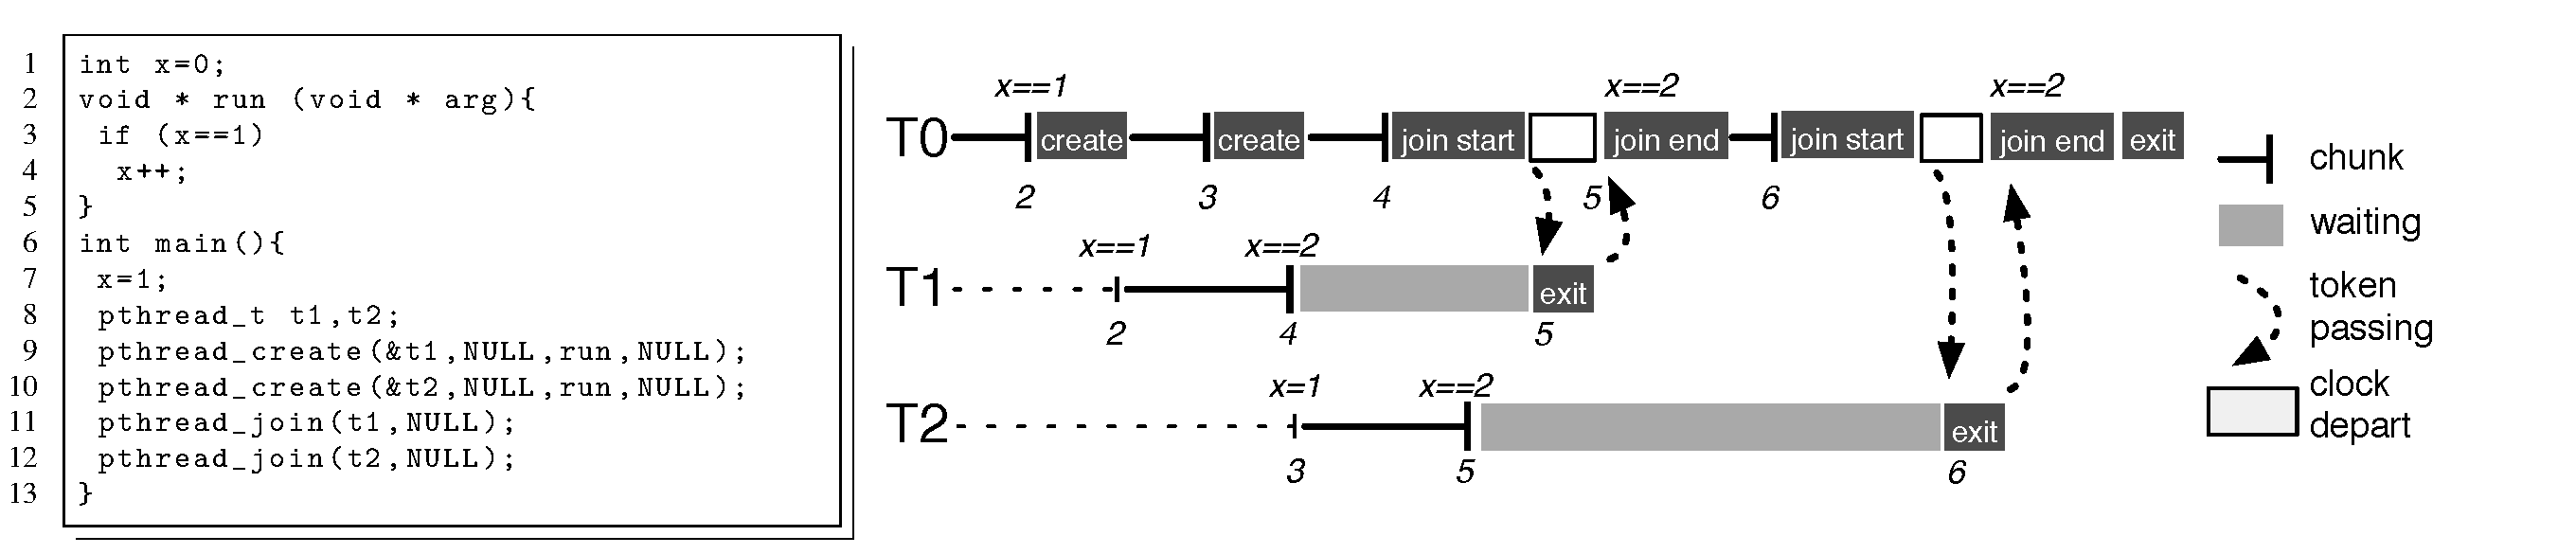
\includegraphics[width=7.25in]{figures/sample_execution}
%\caption{A deterministic execution of a simple program with \lib{}}
%\label{f:sample-execution}
%\end{figure*}

%
%Figure \ref{f:sample-execution} demonstrates the deterministic execution of a simple program using \lib{}. The initial thread T0 begins with its deterministic logical clock (shown as $DLC$) set to 0 and executes its first chunk, terminating when it invokes $pthread\_create$.

%with an equivalent operation surrounded by a pthread lock/unlock, we can regain the lost atomicity.

%\lib{} supports ad hoc synchronization by setting a bound on the number of instructions that can be executed inside a chunk. Once that bound is hit, the thread must perform a commit operation. For the example above, $t_1$ will no longer spin infinitely and will ultimately reach the bound, perform a commit and see $t_2$'s update to $flag$.  

%However, implementing this mechanism for a system with a logical clock built on hardware performance counters is not straightforward. The difficulty derives from the non-deterministic arrival of an interrupt from a counter overflow. If we set the counter to overflow after $n$ events (retired instructions), then the interrupt will arrive after $m$ events where $n \leq m \leq n+interrupt\_window$. The value of \\$interrupt\_window$ is typically informed by the size of the processor's reorder buffer.

%To avoid this non-determinism, we follow the technique introduced in \cite{tom_bergan_deterministic_2010} and set the counter to overflow after $n-interrupt\_window$ events. After receiving the interrupt, we set the processor's trap flag and single step until we reach the desired value of $n$. This ensures a deterministic commit point. Its important to note that we only perform this step when the thread begins to approach the maximum number of instructions that can be executed in a chunk.

%\subsection{Putting it all together: \Lib{} Implementation}
%
%The overall architecture of \lib is shown in \autoref{f:arch}. \lib{} is a fork of the DThreads project \cite{liu_dthreads:_2011} but reimplements the modules that perform deterministic synchronization, memory consistency and other core functionality.\footnote{We reuse the DThreads thread-local heap, shimming support and other basic infrastructure.} For programs linked with \lib{}, calls to pthreads synchronization primitives are instead handled by \lib{}.
%
%\lib{} relies on its deterministic logical clock (DLC) user space library and kernel module for deterministic synchronization. When a thread is spawned, the DLC will create a new logical clock (initialized to the parent's current clock value) and initialize the thread's performance counter to keep logical time. A thread's logical clock is updated at the following times: (a) upon completion of a chunk by reading the performance counter, (b) when a performance counter overflows or (c) when the clock is fast-forwarded (see \S\ref{s:fast-forward}). For the current GMIC thread, any clock update triggers an operation to check whether or not it is still the GMIC.  


%%% Local Variables: 
%%% mode: latex
%%% TeX-master: "paper.tex"
%%% End:

%\section{Background: Deterministic Execution}

Current deterministic execution systems \cite{liu_dthreads:_2011,merrifield_conversion:_2013,kai_lu_efficient_2014} allow an arbitrary multi-threaded program written in a conventional parallel programming language (like C or Java) to execute in a deterministic manner. The program's output and succession of internal states become solely a function of the program's explicit inputs and are unaffected by the nondeterministic interleaving of shared memory operations or OS scheduling decisions.

Determinism is achieved by keeping each thread's memory isolated from other threads', thereby converting a multi-threaded program into a collection of single-threaded programs, each of which are inherently deterministic. Periodically, threads are allowed to communicate with each other by \emph{retrieving} remote updates and \emph{committing} their local updates to make those updates available to remote threads. Previous systems have optimized the performance of this general approach along two main axes: 1) by increasing flexibility in when commits occur and 2) by reducing the number of remote threads that commits are made visible to (i.e., relaxing the memory consistency model).

\begin{figure}
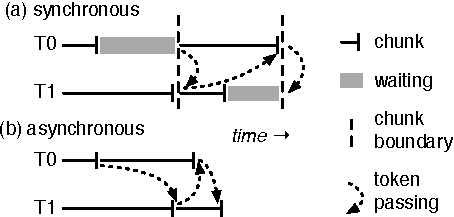
\includegraphics[width=3.0in]{figures/sync-async-chunks.pdf}
\caption{Synchronous versus asynchronous commit.}
\label{f:sync-async}
\end{figure}

Initial deterministic execution systems divided program execution into chunks consisting of a fixed number of instructions (typically 10-100,000) \cite{devietti_dmp:_2009,bergan_coredet:_2010,derek_r._hower_calvin:_2011} or separated by synchronization operations \cite{liu_dthreads:_2011}. 
After a thread executes one chunk it waits for all the other threads to execute their chunks before proceeding. This \emph{synchronous} approach (\autoref{f:sync-async}a) can lead to excessive waiting as threads often execute instructions or synchronization operations at different rates. An alternative \emph{asynchronous} approach was proposed by Merrifield and Eriksson \cite{merrifield_conversion:_2013} that eliminates global barriers, instead allowing threads to commit independently (\autoref{f:sync-async}b). In both synchronous and asynchronous approaches a global token circulates among threads in a deterministic round-robin order to ensure that commits occur deterministically.

\begin{figure}
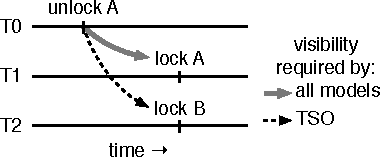
\includegraphics[width=3.0in]{figures/relaxed-consistency.pdf}
\caption{TSO requires that commits are global, while more relaxed models allow local commits that are visible to a subset of threads.}
\label{f:relaxed}
\end{figure}

Relaxing the consistency model improves the performance of determinism by making memory fences cheaper. Memory fence semantics define the number of threads to which commits must be made visible; with weaker consistency this number decreases which reduces the time it takes to push and pull commits. Consistency models like sequential consistency and total store order require that stores become visible in a total order that all threads agree on: commits must thus be a global operation (\autoref{f:relaxed}). Relaxed consistency models like DRF0 \cite{devietti_rcdc:_2011} and LRC \cite{kai_lu_efficient_2014} allow commits to be ``point-to-point'' with respect to a given synchronization object, i.e., the commit performed when releasing a lock need be visible only to the subsequent acquirer of that lock.

Removing global barriers and relaxing consistency offer orthogonal benefits and previous systems have explored these benefits both in isolation and in combination. \cite{merrifield_conversion:_2013} offers TSO with asynchronous commits, the RCDC system \cite{devietti_rcdc:_2011} adopts relaxed consistency but still uses synchronous commits, and RFDet \cite{kai_lu_efficient_2014} provides both asynchronous committing and relaxed consistency.

While RFDet could potentially provide the best performance of these schemes, the adoption of such an extremely relaxed\footnote{It is not obvious how further relaxations beyond LRC would be possible without breaking programming language semantics.} consistency model as LRC entails several additional costs. One concern is a space leak that arises from making commits visible only via a particular synchronization object. If a thread modifies some data and releases lock A, those modifications must be recorded until some other thread acquires lock A. This overhead is incurred for every lock release, causing space usage to scale with the number of lock objects. In the case that no other thread ever acquires lock A, space will be permanently leaked. This space overhead is not just a theoretical concern: in Section \ref{s:rfdet} we report large space overheads for RFDet on a benchmark with only a moderate number of synchronization operations.

 In addition to its space overheads, extremely weak consistency models like LRC are difficult for both humans \cite{adve_data_2010} and automated tools \cite{batty_mathematizing_2011,burckhardt_checkfence:_2007} to understand. The LRC model is substantially weaker than the most relaxed hardware consistency models (POWER and ARM) and thus programs compiled for a stronger model can break when executed on LRC. Recompilation with an LRC-aware compiler is necessary to generate the appropriate memory ordering instructions.

We propose that deterministic systems adopt stronger memory consistency models, such as the TSO model used in this work, to avoid these pitfalls. Next, we give an overview of the \lib system before discussing the optimizations that allow \lib to rival the performance of relaxed consistency approaches.

% We show that deterministic implementations of TSO can outperform weaker models because the cost of pushing and pulling commits can be quite low without resorting to weak consistency \ref{todo}. Furthermore, \textbf{the main performance bottleneck is the cost of deterministic synchronization} which requires centralized coordination in strong and weak consistency models alike. We show in \ref{todo} how to reduce the logical-physical clock skew that makes deterministic synchronization expensive. \TODO{may want to expand on clock skew here}

%%% Local Variables: 
%%% mode: latex
%%% TeX-master: "paper.tex"
%%% End:

%\section{\Lib{} Architecture}

%Synchronization operations like {\tt lock()} and {\tt unlock()}, however, require global coordination. If, as in \autoref{f:local-global}, two threads attempt to perform a {\tt lock()} at the same time, the operations will be deterministically serialized even if the {\tt lock()} calls operate on different locks. 
%One thread can perform local work while another is doing a global operation, however. 
%Thus, the performance of any TSO system can be said to depend on three factors: (a) overhead on local work due to memory isolation and logical clock maintenance, incurred by each thread during its parallel execution or just prior to global coordination; (b) overhead of merging updates which makes global coordination slower; and (c) delays in the transition between local and global phases, due to suboptimal ordering. 

%  The serial phases, meanwhile, are globally serialized and deterministically ordered. Thus, a critical section in \lib{} consists of two serial phases, one each for the {\tt lock()} and {\tt unlock()} operations, and a critical section where the thread operates on its local version. 
% The serial phase that then follows, communicates any changes made to the other threads. 

%In \lib{}, one thread may be performing local work while another is doing a global operation, but to preserve determinism, threads must respect the order in which they enter the serial phase. 

%Since \lib{} implements TSO, all writes need to appear in a total order that all threads agree on irrespective of which locks were held at the time. Compared to more relaxed models TSO may increase the overhead of (b) global coordination as the set of changes communicated between threads is larger. However, overhead on (a) local work and (c) phase transitions remain unchanged with weaker consistency models. Thus, the additional work done to merge updates is the ``performance tax'' of retaining the TSO consistency model.

%It is important to note that an increase in the duration of the global coordination phase has one of two outcomes. If many threads are attempting global coordination simultaneously, making global coordination slower directly impacts the waiting threads and overall performance. Alternatively, if the global phase is not congested, performance need not be significantly impacted. Instead, slower global coordination may merely bring the system closer to the congested state.

%%% Local Variables: 
%%% mode: latex
%%% TeX-master: "paper.tex"
%%% End:

\section{Deterministic Adaptation and Other Means of Performance Improvement}
\label{s:optimizations}

A key insight behind the performance of \lib{} is that deterministic execution does not preclude adaptation on the part of the runtime system. 
Philosophically, a program running under varying conditions cannot be fully deterministic: while the output may be completely deterministic, the time to completion generally is not.
Accordingly, we may adapt to the behavior of the running program, as long as the determinism of program state is preserved. 

In principle, a great number of changes to the underlying execution environment are possible without affecting determinism, either in response to environmental changes or in response to (deterministic) program behaviors. Below, we discuss two such adaptations, followed by three other optimizations used in \lib{}.

%\subsection{Thread Reuse for Fork-Join Programs}
%
%In order to support fork-join programs it is imperative for \lib{} to provide fast thread creation and tear-down. However, the use of processes with private heap and globals segments makes this a challenging goal. When a program invokes \create{}, it effectively forks a new process, and each populated \pte{} in the heap and globals segments must be copied into the child's page table. This can be a large number of entries to copy and adds a significant amount of latency to thread creation. 
%
%To mitigate this effect, we can reuse existing threads that have exited previously during the program. When a thread invokes \create{}, it first checks to see if a thread is waiting in the thread pool. If the pool is empty, a call to \fork{} is initiated; otherwise a thread from the pool is chosen. We prefer to chose a thread that has recently exited over an older thread. The reason for this is that a recently exited thread will have a more recent working copy and thus will require less work by \update{} upon startup. 
%
%Because the stack is not \conversion{}-enabled, a thread taken from the pool will have a stale view of the stack segment. Thus, in order to support stack-allocated arguments to threads, we take a snapshot of the parent's stack and copy it into the child on startup. 


\subsection{Adaptive Coarsening}

\begin{figure*}[t]
\centering
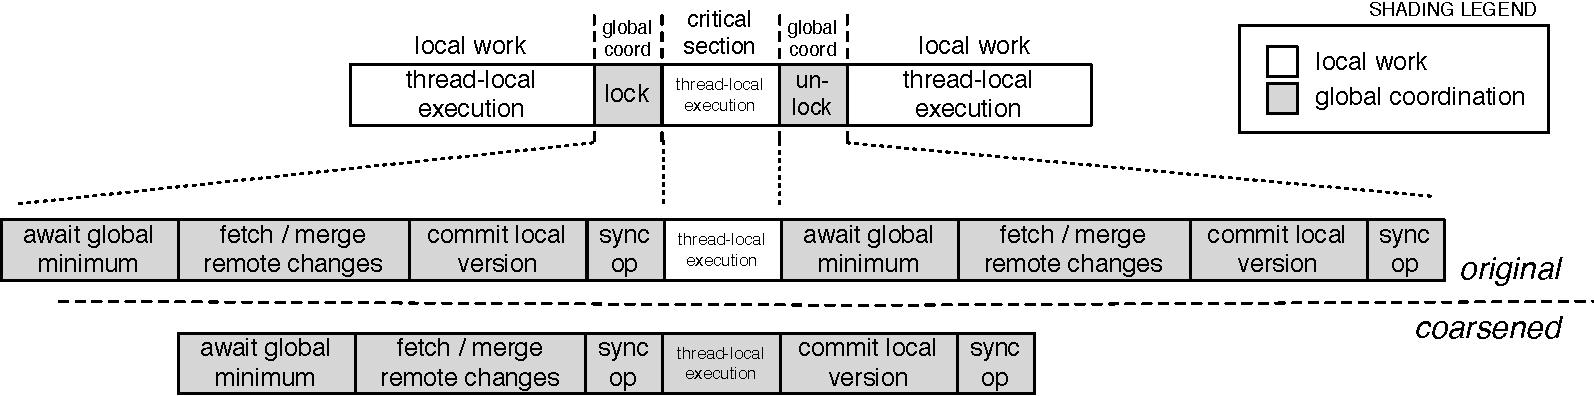
\includegraphics[width=6.8in]{figures/coarsening}
\caption{Program execution under \lib{} is divided into phases of local work and global coordination. In this example, a critical section is surrounded by two phases of global coordination, for the lock and unlock operations respectively. The lower part of the figure shows the result of coarsening on this example.}
\label{f:coarsening}
\end{figure*}

Fig. \ref{f:coarsening} illustrates the operation of \lib{} for a critical section. In the local work phase, all changes are made to the local copy. When a synchronization operation is reached, the thread enters the global coordination phase. It sleeps until it has the global minimum instruction count (GMIC) and can acquire the token, then retrieves any remote updates, and commits its own changes before acquiring the lock. It then releases the token and begins its critical section. The critical section constitutes another local work chunk, which is followed by another global coordination phase. 

From this example, it is clear that though the work performed in the global coordination phase may be highly optimized, each deterministic synchronization operation will incur substantial overhead vs. its nondeterministic equivalent. This problem becomes particularly severe when the time between synchronization operations is brief, such that the local work is dwarfed by the global coordination surrounding it. 

To address this problem, we propose to adaptively reduce the number of global coordination phases, through a technique we call coarsening. In essence, coarsening combines several global coordination phases into a single phase, which includes the intervening local work chunks. The lower part of Fig. \ref{f:coarsening} illustrates the effect of coarsening on a single critical section. Here, the coordination work required is substantially reduced, at the cost of moving what used to be (parallel) local work into the (serialized) global coordination phase. 
As discussed in more detail below, coarsening is not limited to pairs---any number of local work chunks and their surrounding coordination may be coarsened into a single, longer global coordination phase. 

%Recall that a {\it chunk} is a unit of local work that appears between global synchronization phases. 
%When the chunk length is short, the cost of a \lib{} memory fence can become the dominating factor in program execution time. Each memory fence must read the performance counter, wait until its DLC is the global minimum, acquire/release the token and invoke \conversion{} to commit/update/merge memory. For this reason, short chunks can create a significant amount of sequential overhead.

%\TODO{this reads as if we're doing coarsening for everything, but in fact the only coarsening candidates are lock and unlock}

%We can reduce the number of memory fences by coarsening the chunks, creating longer chunk lengths that can effectively mask the overhead of a fence. 
While this technique sounds straightforward, several challenges arise. First, in order to maintain TSO consistency, other threads are blocked at their next synchronization operation until the coarsened chunk has completed. This means that an overly ambitious coarsening policy, producing excessively long coarsened chunks, can significantly harm the overall system by causing excessive waiting of other threads. Second, the choice of when to begin a coarsened chunk must be an informed one. If \lib{} chooses to coarsen and the next chunk is very long (which cannot be known ahead of time) the result would be a net loss in performance. Finally, these decisions need to be done deterministically.

Our approach is to use an adaptive coarsening policy that estimates, for each synchronization variable, the next chunk length using an exponentially weighted moving average of earlier chunk lengths. One such estimate is maintained per lock, for use with coarsening $lock$ operations, and a thread-local estimate is maintained for use with coarsening $unlock$ operations.  
%On completion of a chunk we add the length to a thread-local exponentially weighted moving average (EWMA). Before we execute a memory fence and begin the next chunk we consult the EWMA for a guess of what the next chunk length will be. 
Coarsening proceeds until either (a) the estimated total coarsened chunk length exceeds a maximum threshold, or (b) a conditional variable or barrier operation is encountered. 
%If $current\_length+chunk\_length\_estimate < max\_coarsening\_length$ then we will elide the memory fence and continue. 
%For more accurate statistics we use the synchronization variable as additional context by storing per-variable EWMA's. 

We deterministically adapt the maximum chunk length at runtime, using a multiplicative increase, multiplicative decrease policy. 
Each time a thread $T1$ enters the global coordination phase, $T1$ compares its thread id to the id of the thread $T2$ that previously entered the global coordination phase.
If $T1==T2$, the maximum chunk length is doubled. Conversely, if $T1\neq{}T2$, the maximum chunk length is halved. 
This allows each thread to individually adapt to current conditions.
Because all decisions are based on chunk lengths and the token order, both of which are deterministic, coarsening maintains determinism.

\subsection{Adaptive Counter Overflows}

A thread's logical clock can be updated primarily in one of two ways: (1) when a thread finishes a chunk and the performance counter is read and (2) when a performance counter overflows, triggering an interrupt. Regarding the latter, the choice of overflow frequency is a trade-off between sequential overhead and logical clock accuracy. With a low frequency of overflows, a thread that is not the GMIC may wait longer to receive the notification that they are the new global minimum. However, if the frequency is too high, the cost of exception handling can become unwieldy (see \cite{olszewski_kendo:_2009} for further discussion). 

Our solution to this problem is based on the observation that overflow frequency does not impact determinism at all. A lower or higher frequency may impact when a thread is notified in real time, but it has no bearing in logical time. Therefore,  we design our logical clock module to adapt our overflow frequency using three simple rules. First, at the beginning of each chunk, the overflow is set to a conservative base value of 5,000 retired instructions. Second, if we are the GMIC, then at the beginning of each chunk and at each overflow we check to see if the next lowest logical clock is currently waiting to become the GMIC. If so, we set the performance counter to overflow just when our clock exceeds theirs. Third, if there is not a thread that we must notify then we double the number of instructions that will occur before the next overflow. 

%\subsection{Other Optimizations}

\subsection{Thread Reuse for Fork-Join Programs}

In order to support fork-join concurrency it is imperative for \lib{} to provide fast thread creation and tear-down. However, the use of processes with \conversion{} memory makes this a challenging goal. When a new thread is spawned the call is intercepted by \lib{} and instead a new process is forked (\S\ref{s:isolation}). Because \conversion{} memory is mapped as a private segment, each populated page-table entry in the \conversion{} segment must be copied into the child's page-table. Depending on the application, this can be a large number of entries to copy and adds a significant amount of latency to thread creation. To help mitigate this issue, \lib{} keeps a pool of threads that have recently finished executing. When spawning a new thread, if a thread is waiting in the pool that thread is reused, eliminating an expensive fork operation. The newly spawned thread will still have to update its view of memory to reflect what has been committed since it began waiting in the pool. However, this is typically a much cheaper operation than forking a new process.

\subsection{User Space Reading of Performance Counters}

Our deterministic logical clock module resides primarily in the kernel. One advantage of this approach is that performance counter overflows that identify a new GMIC can notify waiting threads directly from kernel space using shared memory, avoiding costly signals to user space for each overflow. There is added cost to this design however, as \lib{} would require system calls at the end of each chunk to read the counters and determine (and potentially notify) a newly-appointed GMIC thread. To avoid the system call latency for short chunks, we allow user space reading of the performance counters when executing a coarsened chunk.

\lstset{numbers=left,language=C, basicstyle={\footnotesize\ttfamily},tabsize=1,frame=shadowbox,linewidth=7cm,numbers=left}

\newsavebox{\mutexLock}
\begin{lrbox}{\mutexLock}% Store first listing
\begin{lstlisting}
void mutexLock(lock_t* l){
	clockPause();
	while(true){
		waitToken();
		if (lockAcq(l)){;
			convCommitAndUpdateMem();
			break;
		}
		else{
			clockDepart();
			insert(l->waitQueue, _tid);
			releaseToken();
			waitForRelease(l);
		}
	}
	releaseToken();
	clockResume();
}
\end{lstlisting}
\end{lrbox}


\newsavebox{\waitToken}
\begin{lrbox}{\waitToken}% Store first listing
\begin{lstlisting}
void waitToken(){
	while(!isGMIC() || token!=NULL){}
	token=_tid;
}

void releaseToken(){
	token=NULL;
}
\end{lstlisting}
\end{lrbox}

\begin{figure}
\hspace*{.5cm}
\usebox{\mutexLock}
\caption{mutexLock() implementation.}
\label{f:mutexLock}
\end{figure}


\begin{figure}
\hspace*{.5cm}
\usebox{\waitToken}
\caption{A simplified implementation of token acquisition and release.}
\label{f:waitToken}
\end{figure}


\subsection{Fast Forward}
\label{s:fast-forward}

A thread may wait on a conditional variable or lock for an indefinite amount of time, causing its logical clock to become further and further behind the rest of the threads in the system. When the thread is finally woken and acquires the token, it may be the GMIC thread for a long time to come. To combat this, \lib{} ``fast forwards'' a thread's logical clock to the value of the logical clock of the last thread to release the token if that thread had a larger clock.\footnote{Kendo \cite{olszewski_kendo:_2009} employed a similar mechanism to avoid excessive logical clock increments in their locking algorithm.} 

%%% Local Variables: 
%%% mode: latex
%%% TeX-master: "paper.tex"
%%% End:







% ======= STORE/BOX LISTINGS =======



\newsavebox{\mutexUnlock}
\begin{lrbox}{\mutexUnlock}% Store second listing
\begin{lstlisting}
void mutexUnlock(lock_t* l){
	clockPause();
	waitToken();
	lockRelease(l)
	if (!queueEmpty(l->waitQueue)){
		int tid=remove(l->waitQueue);
		wakeupThread(tid);
	}
	convCommitAndUpdateMem();
	releaseToken();
	clockResume();
}
\end{lstlisting}
\end{lrbox}

\newsavebox{\codeSample}
\begin{lrbox}{\codeSample}% Store second listing
\begin{lstlisting}
int x=0;
void * run (void * arg){
	if (x==1)
		x++;
}
int main(){
	x=1;
	pthread_t t1,t2;
	pthread_create(&t1,NULL,run,NULL);
	pthread_create(&t2,NULL,run,NULL);
	pthread_join(t1,NULL);
	pthread_join(t2,NULL);
}
\end{lstlisting}
\end{lrbox}


%\begin{figure}
%\hspace*{.5cm}
%\usebox{\codeSample}
%\caption{A simplified implementation of token acquisition and release.}
%\label{f:waitToken}
%\end{figure}


\section{Synchronization Primitives}
\label{s:sync}

\lib{} supports deterministic versions of mutual exclusion, conditional variables and barriers. As in previous systems \cite{olszewski_kendo:_2009,kai_lu_efficient_2014}, \lib{} uses the GMIC to deterministically order synchronization along with thread creation, exit and join events. Once a thread becomes the GMIC, it is eligible to acquire the \emph{global token} which is required to perform any deterministic event. The token is useful as both an abstraction for maintaining determinism as well as a means of relaxing the traditional GMIC invariant, necessary to perform the coarsening optimization (see \S\ref{s:optimizations}).


\subsection{Mutual Exclusion}

In Kendo \cite{olszewski_kendo:_2009}, in order to ensure progress for others and to avoid introducing deadlocks, a GMIC thread that failed to acquire a lock would repeatedly increment their logical clock by some value until they were no longer the GMIC. This approach suffers from two problems: 1) the choice of a sensible value to add to the clock while polling requires program-specific tuning and 2) many polling requests to check whether there is a new GMIC thread to notify adds needless latency. A better approach would allow the GMIC thread to block and wait for the lock to be released while continuing to ensure progress for others. We accomplish this by adding the ability for a thread to remove itself from GMIC consideration through the $clockDepart()$ function. 

The $mutexLock()$ implementation (shown in Figure \ref{f:mutexLock}) begins by pausing the clock and acquiring the token via the $waitToken()$ function (shown in Figure \ref{f:waitToken}). If the lock is available (Figure \ref{f:mutexLock}, line 6), the thread commits its changes to memory and begins executing its critical section. However in the case of a held lock (Figure \ref{f:mutexLock}, line 10) the thread will remove itself from consideration for the GMIC and add itself to the lock's queue of waiters.

\begin{figure}
\hspace*{.5cm}
\usebox{\mutexUnlock}
\caption{mutexUnlock() implementation.}
\label{f:mutexUnlock}
\end{figure}


Figure \ref{f:mutexUnlock} shows the implementation of $mutexUnlock()$. After pausing the clock and acquiring the token, we check to see if there are any threads waiting for the lock (Figure \ref{f:mutexUnlock}, line 5). If so, we remove the thread from the wait queue and invoke $wakeupThread()$ which activates the thread using a (non-deterministic) conditional variable and adds the thread back into consideration for the GMIC. \footnote{Our simplified code in Figure \ref{f:mutexUnlock} does not handle one case of potential non-determinism. If the newly activated thread is the GMIC, then we must pass the token to them directly to avoid potential non-determinism with the thread that was the GMIC thread prior to activation.}

Note that, unlike in Kendo \cite{olszewski_kendo:_2009}, $mutexUnlock()$ must acquire the token, as it performs a commit. Kendo assumes that applications are data-race-free and thus enforces no isolation between threads.




%Activating a thread in the manner described thus far can create a non-deterministic schedule. For example, a thread $T1$ with a logical clock $n$ is currently the GMIC and is waiting for the token to be released (line 7 of Figure \ref{f:waitToken}). If another thread $T2$ with a logical clock value of $n-1$ is activated by thread $T3$ using $wakeupThread()$ - once thread $T3$ releases the token it can be acquired by either $T1$ or $T2$. To resolve this non-determinism we add an additional shared variable: the \emph{activation sequence number}. Whenever a token-holder activates another thread (both when unlocking a mutex and signaling with a conditional variable), the sequence number is incremented (line 6 of Figure \ref{f:mutexUnlock}. After acquiring the token a thread must check that the sequence number has not changed (line 10 of Figure \ref{f:waitToken}); and if it has the thread must call $clockIsGlobalMinimum()$ again to ensure it is still the GMIC. 

The techniques described above are also used to support deterministic conditional variables.

\subsection{Barriers}

\lib{} takes advantage of barrier semantics and \conversion{}'s parallel commit feature to improve performance. This is not to be confused with prior synchronous deterministic systems, which used \emph{internal} barriers to perform commits from different threads in parallel \cite{bergan_coredet:_2010,jooybar_gpudet:_2013}.

In the case of multiple concurrent committers, \conversion{} may commit pages of memory in parallel through a two phase commit process. The first phase is done in serial, and %allows a thread to acquire ownership of a page, or simply register interest in the page if it is contended. In short, this phase 
determines the order in which changes to each page will be committed. In the second phase, pages are then merged and committed in parallel.
 The work done in phase two is several times larger than that of phase one, leading to better performance through parallelism. 
See \cite{merrifield_conversion:_2013} for more details.

%In order to exploit this mechanism and still maintain determinism, we separate the single commit operation into two separate operations that mirror the phases described above. 
To guarantee a deterministic ordering for our barrier, threads hold the token during phase one. % access to phase one is ordered by token acquisition. % is preceded by token acquisition. %guarded by the deterministic logical clock. 
%When each thread arrives at the barrier it first acquires the token, which establishes its deterministic order of arrival. %After establishing this {\it per-thread} ordering, each thread waits for all prior threads to finish phase one of the commit, thus establishing a {\it per-page} ordering. 
%After this time, threads can safely perform the more costly second phase of the commit in parallel. 
 After completing phase two in parallel, each thread waits at a non-deterministic (pthreads) barrier until all threads have finished committing. All threads then perform an update to get the latest version of memory.


%While \conversion{} has the ability to commit unique blocks of memory (at a page granularity) in parallel, it does not support any mechanism for ensuring a deterministic order of commits. In order to provide both a deterministic \emph{and} parallel commit we add a $linearized\_version$ field to \conversion{}'s metadata accessible both in kernel space and user space. When \conversion{} begins a parallel commit it first acquires a lock and performs an operation which linearizes the commit before proceeding to do the actual commit work (see \cite{merrifield_conversion:_2013} for more details \TODO{on \conversion{}?}). By writing the new version number to the $linearized\_version$ field, a thread in user space can monitor this value and ensure they do not invoke $convCommitAndUpdateMem()$ until a previous version has been linearized.

%\TODO{The below paragraph feels like we're skipping some crucial details. Would a figure help perhaps?}
%We make use of this new feature in our barrier implementation as follows. When each thread arrives at the barrier it first acquires the token, which establishes its deterministic order of arrival. While holding the token, the thread reserves a future version $V_i$ of memory for their own commit and then releases the token.\footnote{The final thread arriving at the barrier will hold on to the token in order to prevent non-determinism from memory commits by threads not arriving at the barrier.}   The thread then monitors the $linearized\_version$ field, waiting until all versions $V_j$ s.t. $V_j<V_i$ have been linearized. Once this has occurred the thread can safely call $convCommitAndUpdateMem$ and commit its version. After this phase each thread waits at a non-deterministic barrier until all threads have finished their commit. At this time, a final update of memory is needed so that each thread gets the latest version of memory committed by the last thread in the barrier. 

%
%
%
%
%
%\begin{figure*}
%\centering
%
%\begin{subfigure}[Figure A]{}
%\begin{lstlisting}
%void mutexLock(lock_t* l){
%	clockPause();
%retry:
%	waitToken();
%	bool gotLock=lockAcq(l)
%	if (gotLock==true){;
%		commitAndUpdateMem();
%	}
%	else{
%		if (failed++ == 0)
%			commitAndUpdateMem();
%		clockDepart();
%		queueInsert(l->waitQueue, _threadEntry);
%		releaseToken();
%		waitForRelease(l);
%	}
%	clockResume();
%}
%\end{lstlisting}
%\end{subfigure}
%
%\begin{subfigure}[Figure B]{}
%\begin{lstlisting}
%void mutexUnlock(lock_t* l){
%	clockPause();
%	waitToken();
%	lockRelease(l)
%	if (!queueEmpty(l->waitQueue)){
%		wakeupThread(queueRemove(l->waitQueue));
%	}
%	commitAndUpdateMem();
%	releaseToken();
%	clockResume();
%}
%\end{lstlisting}
%\end{subfigure}
%
%\end{figure*}

%%% Local Variables: 
%%% mode: latex
%%% TeX-master: "paper.tex"
%%% End:

\section{Evaluation}
\label{s:eval}

\begin{figure*}
\centering
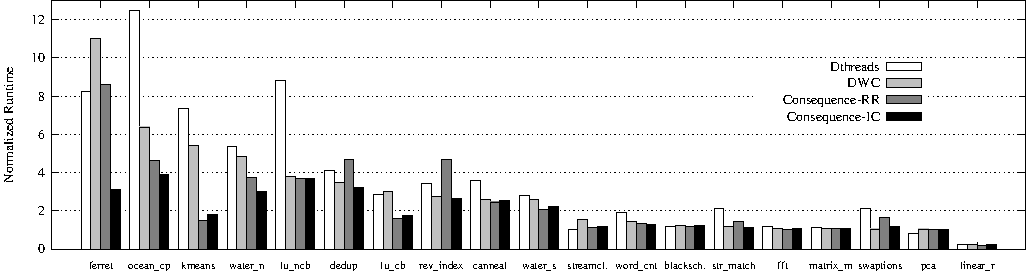
\includegraphics[width=7.0in]{figures/overall_runtimes.pdf}
\caption{\lib{}, DThreads and DWC runtime normalized to pthreads runtime. Main result shown as \lib{}-IC. \lib{}-IC achieves an average of 2.8$\times$ and 2.2$\times$ improvement over DThreads and DWC (respectively) on the five most challenging benchmark programs.}
\label{f:performance}
\end{figure*}

\begin{figure*}
\centering
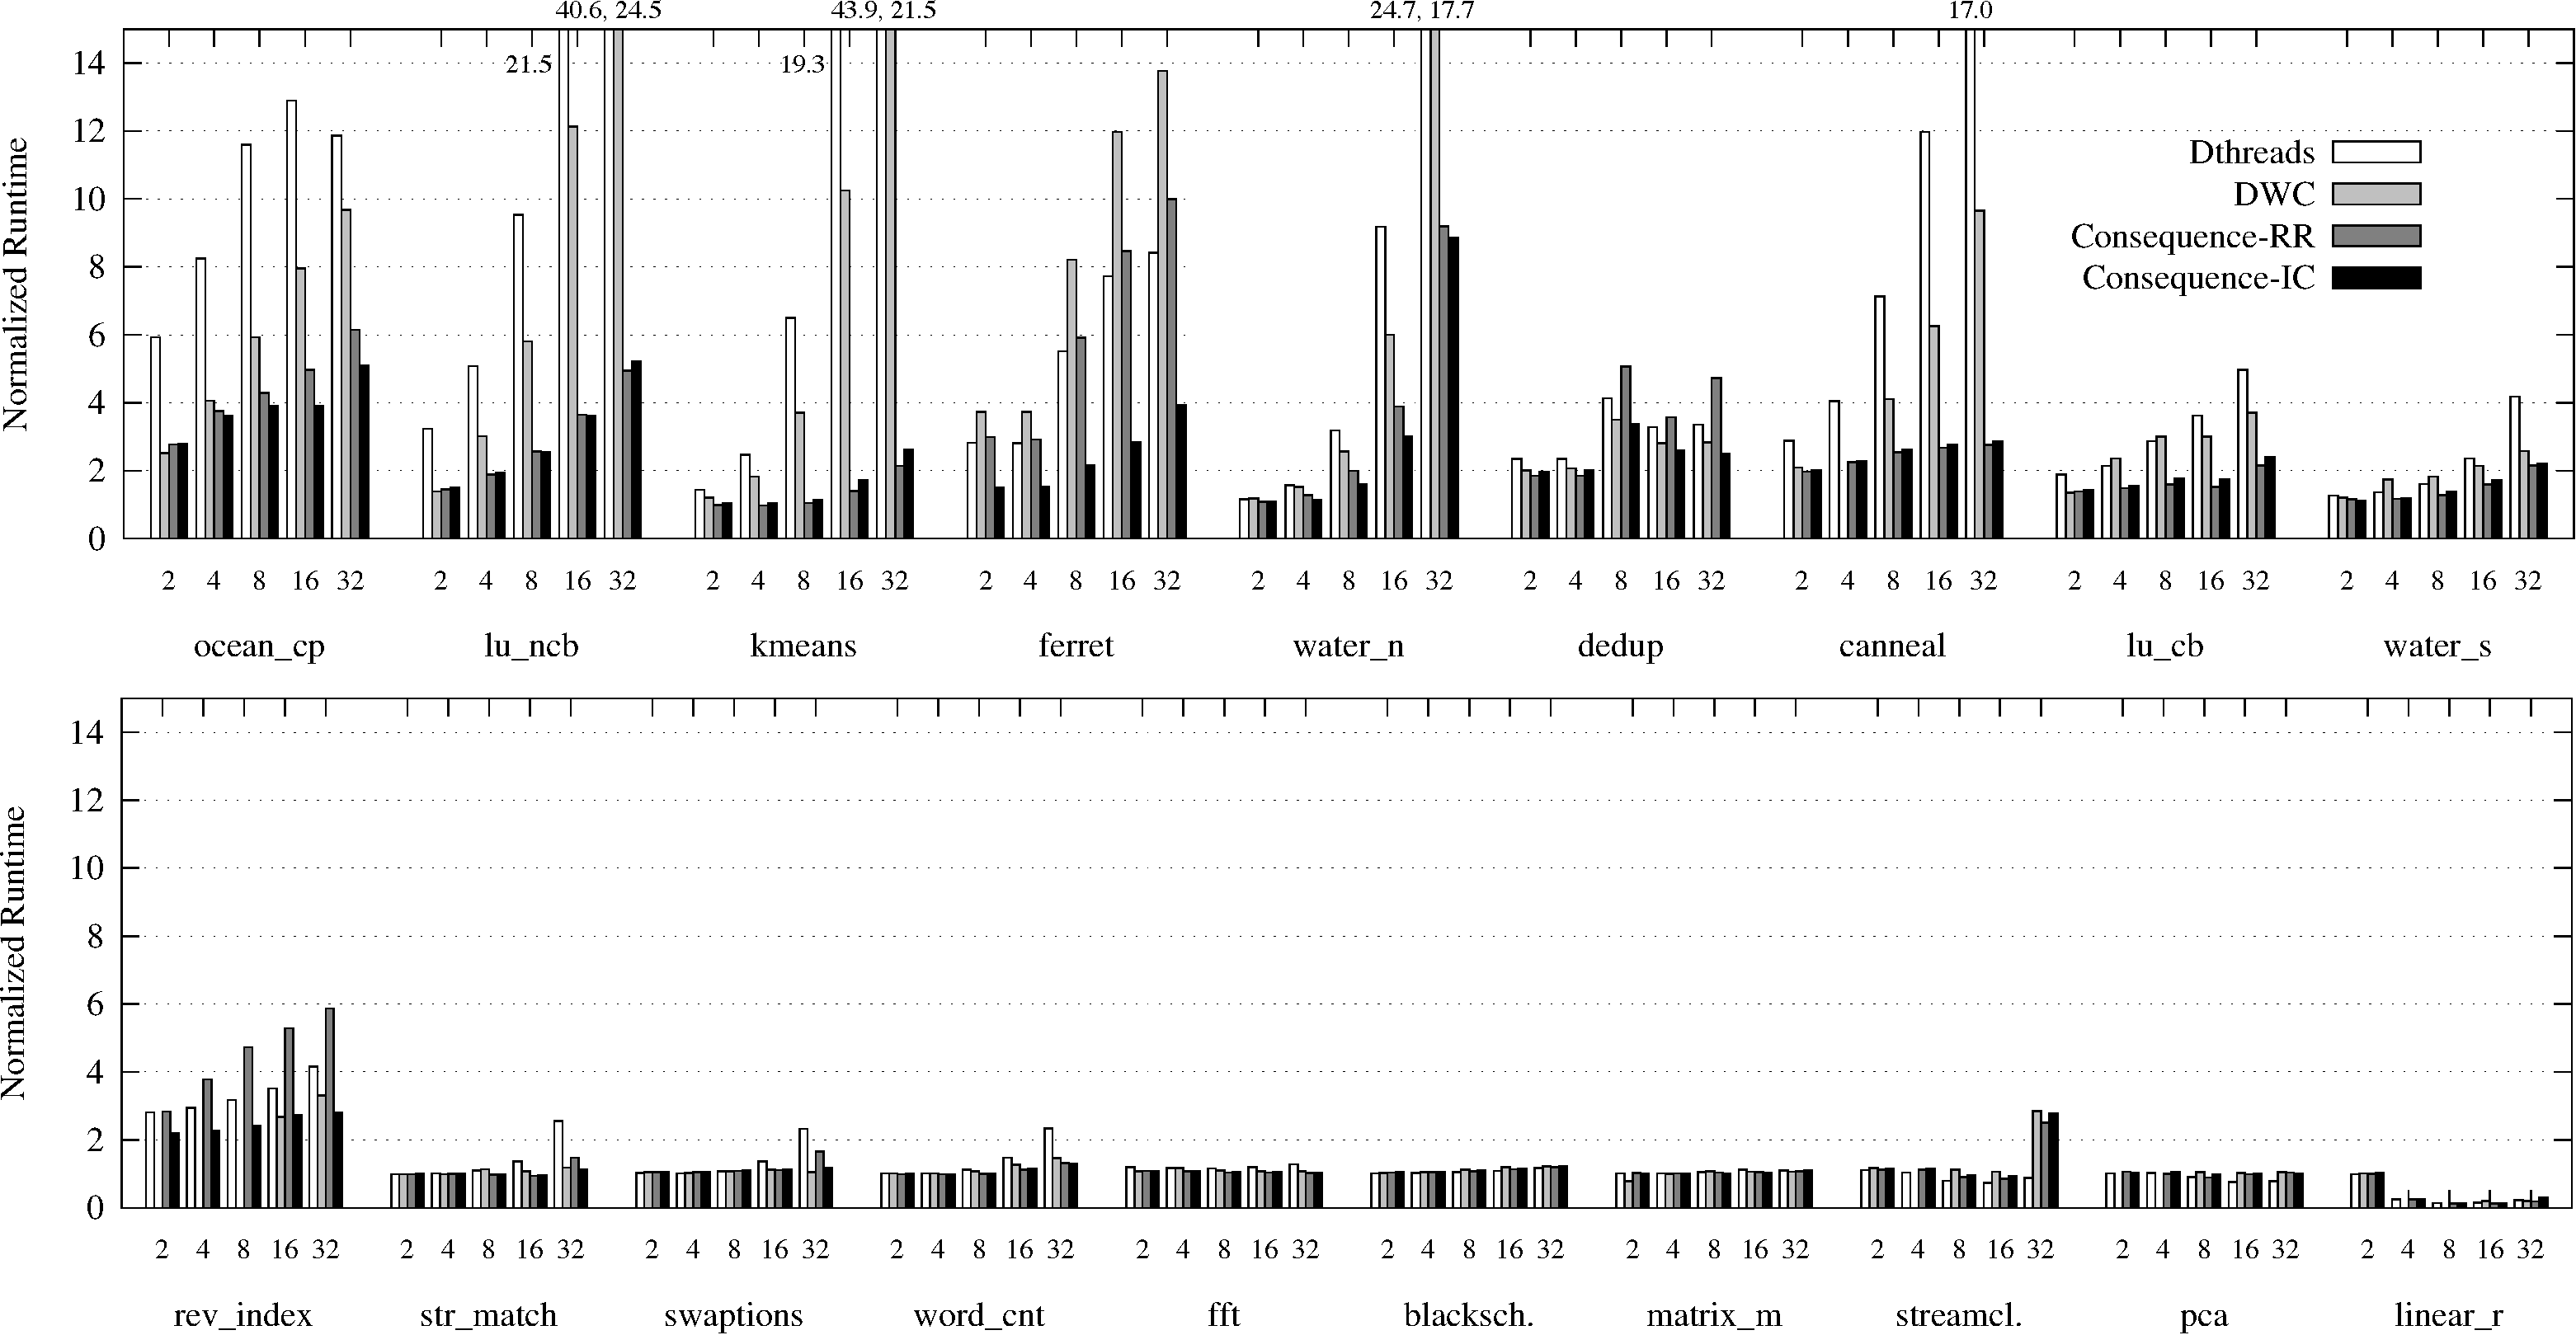
\includegraphics[width=7.0in]{figures/scalability_results.pdf}

\caption{Performance when varying the number of threads for \lib{}, DThreads and DWC.}
\label{f:scalability}
\end{figure*}

\begin{figure*}
\centering
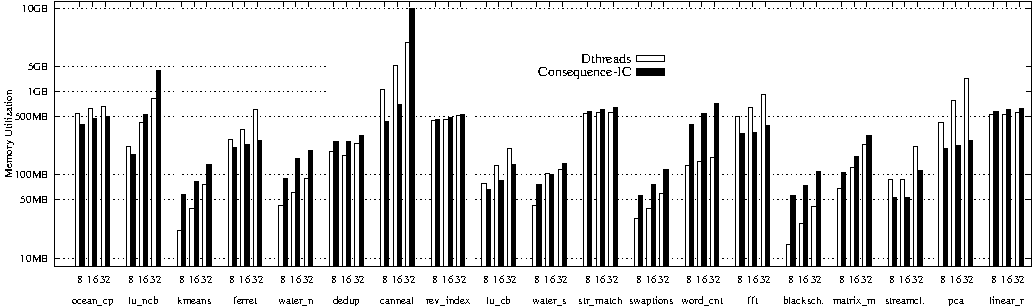
\includegraphics[width=7.0in]{figures/memory_utilization.pdf}
\caption{Peak memory usage for \lib{} and DThreads.}
\label{f:memory}
\end{figure*}

Below, we study the performance of \lib{} in broad strokes, followed by several detail studies. Our results were produced on a computer with four 2.00GHz Intel Xeon E7-4820 8-core processors and 256GB of main memory, running Linux 2.6.37 with the \conversion{} and \lib{} kernel patches. For these experiments, Hyper-threading was turned off, and the frequency scaling governor was set to \emph{performance}. Experiments were run 10 times per thread count, and mean deviation was within 20\% for all benchmarks other than {\it linear\_regression}, where the execution times can be below 500ms.

Figure \ref{f:performance} illustrates our main result: the runtime of two different variations of \lib{}, as well as DThreads \cite{liu_dthreads:_2011} and DThreads with \conversion{} (DWC) \cite{merrifield_conversion:_2013}. \footnote{Unfortunately a comparison with the relaxed consistency system RFDet \cite{kai_lu_efficient_2014} was not possible as the current implementation is provided without deterministic synchronization.} DThreads and DWC both use round-robin ordering, commits at synchronization operations and virtual memory-based isolation through either {\tt mprotect()} (DThreads) or specialized kernel support (DWC). For each library we present results from 19 benchmarks\footnote{Other benchmark programs from Parsec, Phoenix and SPLASH-2 are problematic for deterministic execution. This is mainly caused by the use of ad-hoc synchronization techniques. See \cite{liu_dthreads:_2011} for details.} from the Phoenix, Parsec and SPLASH-2 benchmark suites, normalized to pthreads runtime. 

To produce this plot, we measured the performance of each library (as well as pthreads) using 2--32 threads, and retained the corresponding best result. The plot shows the best library runtime, divided by the best pthreads runtime, for each benchmark. 

Here, \lib{}-RR uses round-robin ordering based on synchronization operations (similar to that used in DThreads and DWC), while \lib{}-IC uses GMIC ordering (see \S\ref{s:dlc}). We see a maximum slow-down vs. pthreads of 3.9$\times$ using \lib{} with the deterministic GMIC ordering (compared to 12.5$\times$ with DThreads and 11.0$\times$ with DWC). The maximum slow-down is arguably the number to watch, as many of the benchmarks are ``embarrassingly parallel'' to start with and offer little or no insight into the performance of these libraries. While DThreads and/or DWC do outperform \lib{}-IC on some benchmarks, this difference is within the mean variation for all but two programs: {\it linear\_regression} and {\it pca}. Further, all cases where a \lib{} variant is not the top performer occur for programs where the max slow-down is less than 2.0$\times$ pthreads across all libraries. 

An interesting result occurs on the {\it reverse\_index} and {\it dedup} benchmarks, where \lib{} is negatively impacted by its more sophisticated and flexible locking algorithm. Both DThreads and DWC treat each lock as a single global lock, which works well for programs where there is only a single lock and critical sections are short. This causes \lib{}-RR performance to suffer, yet \lib{}-IC still manages to provide the best performance by generating a better deterministic ordering.

Figures \ref{f:scalability}--\ref{f:memory} analyze the scalability of \lib{} with respect to thread count, in terms of runtime and memory usage. These reveal a severe DThreads and DWC scalability problem for six benchmarks: {\it  ocean\_cp, lu\_ncb, ferret, kmeans, water\_nsquared} and {\it canneal}. \lib{} also exhibits scaling difficulties, albeit much less severe. 

On the {\it water\_nsquared} benchmark with 32 threads, \lib{} experiences a drastic and unexpected performance hit. This occurs because each thread performs many fine-grained lock acquisitions with short critical sections, which become coarsened with \lib{}. Because a thread holds on to the token throughout the entire coarsened chunk, other threads may be blocked, leading to the scalability issue seen here.

In terms of memory usage (see Figure \ref{f:memory}), DThreads and \lib{} appear evenly matched. Two notable exceptions are {\it canneal} and {\it lu\_ncb} at high thread counts. This is caused by a high volume of page allocation/freeing such that the single-threaded \conversion{} garbage collector cannot keep up. A multi-threaded collector would solve this issue.

\subsection{Sources of Performance Improvement}

As described in \S\ref{s:optimizations}, \lib{} includes a number of performance optimizations, aimed at reducing the cost of common concurrency patterns. To better understand how these various parts contribute to the performance of \lib{}, we evaluate \lib{}-IC with and without each of these optimizations.

\begin{figure}
\centering
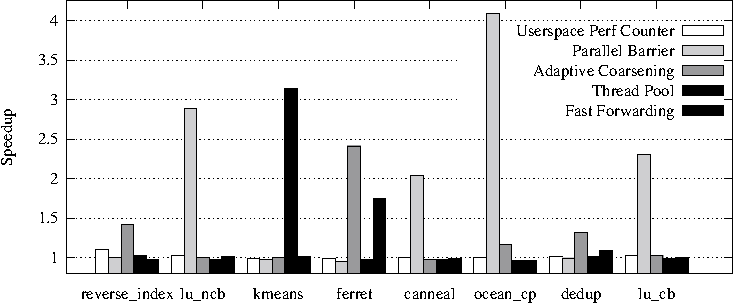
\includegraphics[width=3.3in]{figures/optimizations.pdf}
\caption{Speedup (higher is better) of various optimizations on a select group of benchmarks.}
\label{f:optimizations}
\end{figure}

Figure \ref{f:optimizations} shows the performance improvement (higher is better) contributed by each of five major optimizations, on eight of the most difficult benchmarks. While all optimizations demonstrate some amount of improvement, we find that user space performance counter readings contribute very little to the overall performance. For {\it ferret}, being one of the hardest of the benchmark programs to perform well on, both the adaptive coarsening and fast forward optimizations provide major speed improvements. For {\it ocean\_cp, lu\_ncb, canneal} and {\it lu\_cb} the parallel barrier provides the main source of our speedup. Note that these numbers represent the performance difference in \lib{} with and without each optimization, not a performance improvement with respect to pthreads or DThreads. 


\begin{figure}
\centering
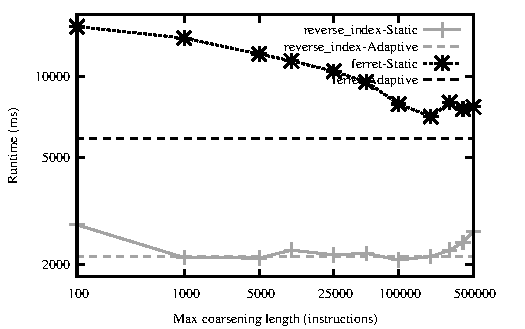
\includegraphics[width=3.1in]{figures/adaptive.pdf}
\caption{Comparison of Adaptive and Static Coarsening for {\it reverse\_index} and {\it ferret}. }
\label{f:adaptive}
\end{figure}


Adaptive Coarsening stands out as one of the most successful optimizations, which merits additional study. Figure \ref{f:adaptive}, shows the effect of coarsening level (x-axis) on the runtime (y-axis, lower is better) of the {\it reverse\_index} and {\it ferret} benchmarks. It is clear that the coarsening level has a significant effect of runtime performance, even when set statically. With adaptive coarsening, each thread selects its own coarsening level, allowing adaptive coarsening to outperform even the best statically chosen coarsening level. 

\subsection{What is Holding \Lib{} Back?}
\begin{figure*}
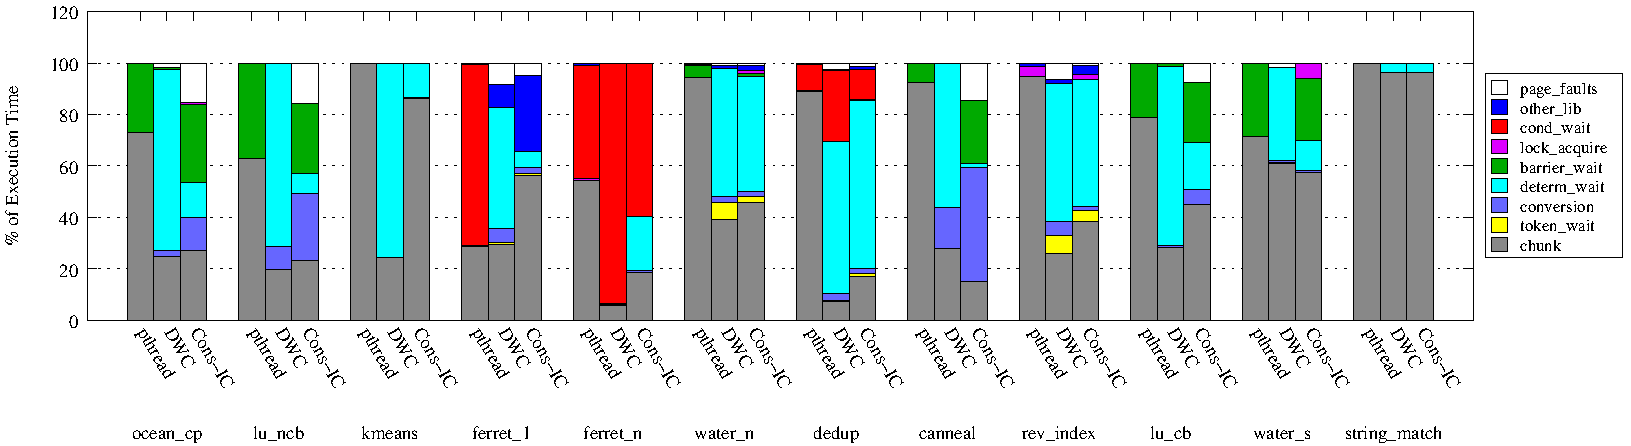
\includegraphics[width=7.0in]{figures/fine_grained_analysis.pdf}
\caption{Breakdown of the time spent in each benchmark with pthreads, DWC and \lib{}-IC using 8 threads.}
\label{f:fine-grained}
\end{figure*}

Figure \ref{f:fine-grained} provides a breakdown of where \lib{} spends time for a selection of benchmarks. The benchmarks can be divided between ``embarrassingly parallel'' ({\it string\_match}), barrier-heavy ({\it ocean\_cp, lu\_cb, lu\_ncb, canneal, water\_nsquared and water\_spatial}) and those that experience other determinism-related overhead ({\it kmeans, ferret, dedup and reverse\_index}). For {\it ferret}, the first thread spawned is presented on its own ({\it ferret\_1}) because it exhibits a radically different synchronization pattern than the rest ({\it ferret\_n}).

For the barrier-heavy programs (e.g. canneal), DWC typically has a much higher execution time (see Figure \ref{f:scalability}) and a large percentage of that time is spent waiting on others. This is because the DWC barrier commits are done serially and the amount of memory that must be committed is typically high. In \lib{}-IC, much of the commit work is done in parallel so the wait time (shown as barrier\_wait\footnote{We separate barrier\_wait and determ\_wait time for \lib{} because the time spent waiting at the barrier is not impacted by deterministic ordering.}) is greatly reduced. With less wait time, the remaining overhead is spread between copy-on-write page faults and commit operations in \conversion{}. For {\it canneal} and {\it lu\_ncb} the time spent in \conversion{} is higher because threads tend to write to the same page in isolation, leading to a larger number of byte-granularity merges.

The {\it ferret} program provides an interesting challenge for deterministic execution. The first phase of the pipeline (shown as {\it ferret\_1}) performs a high volume of lock acquisitions with short chunk sizes, while the rest of the threads oscillate between executing longer chunks and waiting at conditional variables. For good deterministic performance, it is important to (1) provide an ordering that allows the first thread to perform synchronization unimpeded, and (2) reduce the cost of each synchronization operation. \lib{}-IC provides (1) through GMIC ordering and (2) through adaptive coarsening. This results in more time spent executing chunks and less time spent waiting or performing page faults.\footnote{Coarsening can reduce the total number of page faults if two chunks in a coarsened chunk write to the same page.}. \lib{}-IC still experiences a large amount of general library overhead on {\it ferret\_1} which is mainly caused by reading the performance counters and other work done between chunks.

\subsection{Memory Propagation for Relaxed Models}

For some benchmark programs like {\it canneal} and {\it lu\_ncb}, the amount of memory that must be propagated between threads can degrade \lib{} performance. Therefore, it is worth investigating whether relaxed memory models can perhaps alleviate this burden on deterministic execution.

An LRC-based memory model can reduce total memory propagation by allowing commits to be "point to point." More specifically, memory is propagated between threads using the \emph{happens-before} relation. An operation $a$ is said to have happened before $b$ if (1) $a$ occurs before $b$ within the same thread of execution, or (2) $a$ and $b$ are release and acquire operations on the same synchronization variable. 

To evaluate the reduction in memory propagation that a relaxed memory model can offer, we modified \lib{} to track the happens-before relation. This was achieved by adding a vector clock to each thread, synchronization variable and committed page. For each acquire operation (lock, conditional wait, thread creation/join and barrier wait)\cite{kai_lu_efficient_2014}, we compute which pages would need to be propagated along happens before edges.

Figure \ref{f:tsovslrc} compares the total number of pages propagated under TSO (\lib{}) and the expected number for an LRC-based system across 12 benchmarks that perform at least 10K page updates. While the LRC system can reduce total memory propagation, the reduction is just 21\% when averaged across all benchmarks considered. For some benchmarks like {\it canneal}, the use of barriers limits the gains from using a relaxed consistency model.


\section{Related Work}
\label{s:related}

The Kendo \cite{olszewski_kendo:_2009} and Deterministic Shared Memory Multiprocessing (DMP) \cite{devietti_dmp:_2009} systems first showed how to provide determinism for general multi-threaded programs: Kendo was a pure-software system that leveraged performance counters and DMP used hardware support to provide determinism even for programs with data races. Follow-on work has shown a variety of ways to optimize the performance overheads of determinism, e.g., through compiler optimizations \cite{bergan_coredet:_2010}, relaxed memory consistency \cite{derek_r._hower_calvin:_2011,devietti_rcdc:_2011,amittai_aviram_workspace_2011,derek_r._hower_hobbes:_2011}, existing hardware support for virtual memory \cite{berger_grace:_2009,amittai_aviram_efficient_2010,tom_bergan_deterministic_2010,liu_dthreads:_2011}, and eliminating the synchronous implementation of commits present in prior determinism systems \cite{merrifield_conversion:_2013}. Segulja and Abdelrahman \cite{Segulja:2014:pact:cost-weak-det} measure the performance cost of enforcing a deterministic logical clock and find it to be less than 2x across a range of benchmarks and runtime perturbations, showing that determinism needn't be fundamentally expensive. Recently, the RFDet system \cite{kai_lu_efficient_2014} demonstrated the performance benefits of memory consistency optimizations with its deterministic implementation of LRC \cite{keleher_treadmarks:_1994}.

% jld: I didn't mention ddos.

There is also a large body of work on programming languages that enforce deterministic parallelism. These languages ensure determinism by construction, e.g., via data-parallel functional programming models \cite{guy_blelloch_nesl:_1992}, annotations to identify opportunities for parallelism in sequential code \cite{rinard_design_1998}, stream-based programming models \cite{william_thies_streamit:_2002}, or type-and-effect systems for imperative languages \cite{bocchino_type_2009}. Blelloch et al. \cite{shun_brief_2012} describe the \emph{deterministic reservations} programming discipline for scheduling potentially conflicting parallel operations in a deterministic way, showing good speedups on a range of parallel algorithms. The Deterministic Galois system \cite{nguyen_deterministic_2014} shows how to enforce deterministic reservations automatically, guaranteeing deterministic results for all Galois programs. While programs written in these deterministic languages often show good performance and scalability, \lib provides determinism for legacy binary programs and does not require that programs be rewritten or even recompiled.

Another vein of work investigates limiting the nondeterminism of multi-threaded programs through \emph{stable multi-threading}. Instead of forcing every execution of a particular input to deterministically follow the same schedule, a small set of schedules are found that any input can nondeterministically follow. The flexibility to nondeterministically choose a schedule at runtime typically allows for higher performance. Early work on stable multi-threading relied on sophisticated program analysis \cite{heming_cui_stable_2010,heming_cui_efficient_2011,bergan_input-covering_2013} to discover the set of permitted schedules. More recently, the Parrot \cite{cui_parrot:_2013} system eschews such analysis in place of programmer annotations that identify where schedule flexibility is needed. Parrot's limited nondeterminism has been shown to amplify the power of verification techniques like model checking. While \lib does not require programmer annotations to achieve good performance, the authors of \cite{cui_parrot:_2013} observe that stable multi-threading and determinism are not mutually exclusive. In future work we hope to better understand what trade-off exists between stability and determinism.

%%% Local Variables: 
%%% mode: latex
%%% TeX-master: "paper.tex"
%%% End:


\section{Conclusion}

With \lib we demonstrate that highly relaxed memory consistency is not necessary for high-performance deterministic execution; \lib achieves similarly good performance while retaining the stronger TSO consistency model. The performance benefits of relaxed consistency, which allow memory fences to be implemented as local operations, are attenuated by the fact that deterministic synchronization still requires global coordination. We identify performance optimizations for the TSO consistency model that reduce the cost of memory fences and that exploit adaptivity to program behavior while still maintaining determinism. We also propose the first implementation of deterministic locking that supports blocking instead of polling.
We plan to release the source code for our entire system to enable future researchers to duplicate and build upon our results.



%\category{CR-number}{subcategory}{third-level}

% general terms are not compulsory anymore, 
% you may leave them out
%\terms
%term1, term2

%\keywords
%keyword1, keyword2



%\appendix
%\section{Appendix Title}
%This is the text of the appendix, if you need one.
%\acks
%Acknowledgments, if needed.

% We recommend abbrvnat bibliography style.

\bibliographystyle{abbrvnat}

\bibliography{consequence}

% The bibliography should be embedded for final submission.

%\begin{thebibliography}{}
%\softraggedright

%\bibitem[Smith et~al.(2009)Smith, Jones]{smith02}
%P. Q. Smith, and X. Y. Jones. ...reference text...

%\end{thebibliography}


\end{document}

%                       Revision History
%                       -------- -------
%  Date         Person  Ver.    Change
%  ----         ------  ----    ------

%  2013.06.29   TU      0.1--4  comments on permission/copyright notices

